%
% 2009年度版最終課題
%

\section{最終課題 大規模ネットワークの構築}
ネットワーク管理者はこれまで実験で行ってきたような,グループ単位のよう
な小さなLANだけでなく,大規模なネットワークの構築を要求される場合もあ
る.

最終課題として,これまでの実験3・4や講義で培ってきた知識を用い,実験に
参加している全てのグループと共同で一つの大きなネットワークを設計・構築
を行う.ただし,本章では構築するネットワークの概要は予め定めておくが,
詳細な実現方法等についての説明は行わない.各グループで割り当てられた役
割を遂行するために必要な知識は,各々が書籍・マニュアル等で調べる必要が
ある.

\subsection{ネットワーク構成図}
まず,最終課題で構築するネットワークの構成図を図{\ref{final:fig:finalnet}}に示す.
\begin{figure}
\begin{center}
\resizebox{!}{9cm}
    {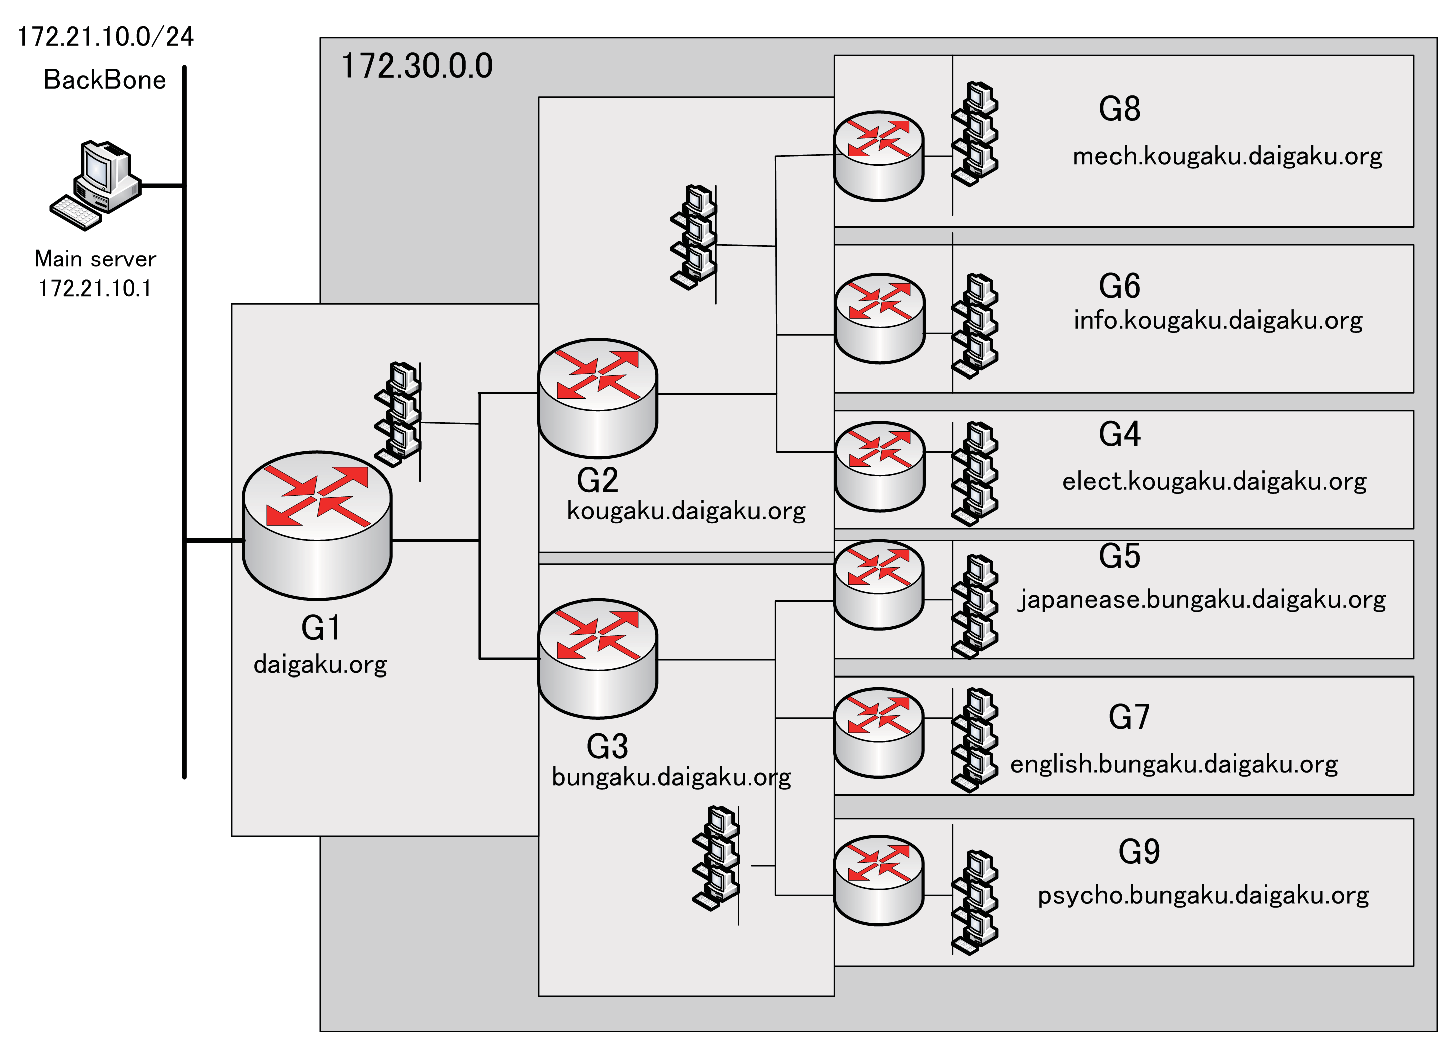
\includegraphics{./etc/specs/final.eps}}
\vspace*{-1zh}
\end{center}
\caption{最終課題構成図}
\label{final:fig:finalnet}
\end{figure}
ただし,ここで使用しているグループやドメインは仮のものであり,どのグルー
プがどこを担当し,どのようなドメイン・サブドメインにするかは後ほど決定
する.

\subsection{要求仕様}

\subsubsection{各グループのIPアドレスの割り当て}
G1以下の全体のネットワークに 172.30.0.0(ナチュラルマスク)のネットワー
クが割り当てられているので,各グループ同士で協議の上,サブネット化をし
て用いる.

\subsubsection{各グループの責任範囲}
各グループが責任を持って設定しなければならない範囲は,各グループのルー
タの上流側インターフェイスの接続・設定から下流側のサブネットワークの全
ての機器(スイッチングハブ,サーバ,コンピュータ,周辺機器,ケーブル)
である.ただし下流側ルータのインターフェイス接続は,下流側グループの担
当となる.

\subsubsection{各グループのルータのIPアドレス}
\begin{itemize}
\item 各サブネットの最も小さい IP アドレスから付与する.
\item サブネット内に複数のルータがある場合は,グループ番号の小さいものから順に付与する.
\end{itemize}

\subsubsection{ルーティング}
\begin{itemize}
\item 静的ルーティングを用いる.
\item 各ワークステーション,コンピュータ等は,デフォルトゲートウェイとして自
グループの上位側ルータを指定する.
\end{itemize}

\subsubsection{DNS ドメインの構成}
\begin{itemize}
\item G1 以下の全体ネットワークに daigaku.org ドメインが付与されている.
\item G1 が daigaku.org ゾーンを管理し,G2,G3 にそれぞれサブドメイン
  kougaku, bungaku を割り当てて,それらのゾーンを委譲する.
\item G2 は kougaku.daigaku.org ゾーンを管理し,G4,G6,G8 にそれぞれ
  elect,info,mech サブドメインを割り当て,ゾーンを委譲をする.
\item G3 は bungaku.daigaku.org ゾーンを管理し,G5,G7,G9 にそれぞれ
  japanese,english,psycho サブドメインを割り当て,ゾーンを委譲をする.
\item G4 は elect.kougaku.daigaku.org ゾーンを管理する.
\item G5 は japanese.bungaku.daigaku.org ゾーンを管理する.
\item G6 は info.kougaku.daigaku.org ゾーンを管理する.
\item G7 は english.bungaku.daigaku.org ゾーンを管理する.
\item G8 は mech.kougaku.daigaku.org ゾーンを管理する.
\item G9 は psycho.bungaku.daigaku.org ゾーンを管理する.
\item 逆引きは考えなくてよい(設定を行う必要はない).
\end{itemize}

\subsubsection{外部ネットワークとの接続}
\begin{itemize}
\item 各グループのサーバ間は,接続可能であること.
\item 各グループのサーバは,Mail server 172.21.10.1 に接続可能であること.
\item 各グループのサーバは,backbone 172.21.10.0/24 に接続可能であること.
\end{itemize}

\subsubsection{サービス}
\begin{itemize}
\item 全ての端末からメール送受信,ウェブ閲覧が行えること.
\item メールアカウントは全員分作成する.
\item その他,必要と感じるサービス,便利であると考えるサービスがあれば
  構築する.構築したサービスについては,レポートに記述すること.
\end{itemize}


\subsubsection*{考慮すべき点}
\begin{itemize}
\item どのようにネットワークの設計を行うか
\item どのような設定をして要求する仕様を満たすか.
\item ネットワークのポリシーはどのように設定すべきか.
\item 他者との共同作業をどのように行うべきか.
\item どこまでが自分の責任範囲で,どこからが他者に責任範囲か.
\item 他者への設定依頼はどのようにすべきか.
\end{itemize}

